% SC4024 --- Chapter 4: Statistical Charts & Interaction (0->100 ground-up)
\chapter{Statistical Charts \& Interaction}
\label{ch:statistical-interaction}
\sloppy

\begin{quote}
\emph{``Overview first, zoom and filter, then details on demand.''} --- Shneiderman's mantra captures the move from static distributions to interactive exploration. This chapter builds that bridge.
\end{quote}

\noindent\fbox{\parbox{\dimexpr\linewidth-2\fboxsep-2\fboxrule}{%
\textbf{From zero: we build here, no prior statistics beyond means needed.} We introduce histograms, KDE, boxplots, and scatter matrices from intuition, then add brushing, linking, and dynamic queries, with small examples and code. No prior stats-visualisation experience is required.}}
\vspace{0.4em}

\section*{Learning Outcomes}
After this chapter you will be able to:
\begin{enumerate}[label=(L\arabic*)]
    \item choose among histogram, KDE, boxplot, violin, and rug for a distribution task;
    \item select bin width and bandwidth and explain their bias--variance trade-off;
    \item design scatterplot matrices and parallel coordinates for multivariate data;
    \item implement brushing, linking, filtering, and details-on-demand;
    \item evaluate interaction latency and visual scalability limits.
\end{enumerate}

% ============================================================
\section{Showing One Distribution}
\label{sec:one-dist}
\paragraph{Intuition.} You have 200 exam scores. A list says little; a picture of how many fall in each interval says a lot. But the picture depends on how you slice the intervals---too wide and you hide bimodality, too narrow and noise dominates.

\paragraph{Formal view.} A \emph{histogram} partitions the range into bins of width $h$ and counts $n_j$ per bin; bar height is $n_j$ (or density $n_j/(nh)$). A \emph{kernel density estimate} smooths: $\hat{f}_h(x)=\frac1{nh}\sum K((x-x_i)/h)$ for kernel $K$ (Gaussian). Histogram is a box kernel on bin centres; KDE is its smooth limit. A \emph{boxplot} shows median, quartiles $Q_1,Q_3$, IQR, whiskers to $1.5\,\text{IQR}$, and outliers. \emph{Violin} adds a mirrored KDE; \emph{rug} marks each point.

\begin{definition}[Bin and bandwidth rules]\label{def:bin-rules}
Heuristics: Sturges $k=\lceil\log_2 n+1\rceil$ bins; Scott $h=3.5\sigma n^{-1/3}$; Freedman--Diaconis $h=2\,\text{IQR}\,n^{-1/3}$ (robust to outliers). For KDE, bandwidth $h$ trades bias (oversmooth, hides peaks) vs variance (undersmooth, wiggles). Leave-one-out cross-validation can tune $h$.
\end{definition}

\begin{figure}[h]\centering
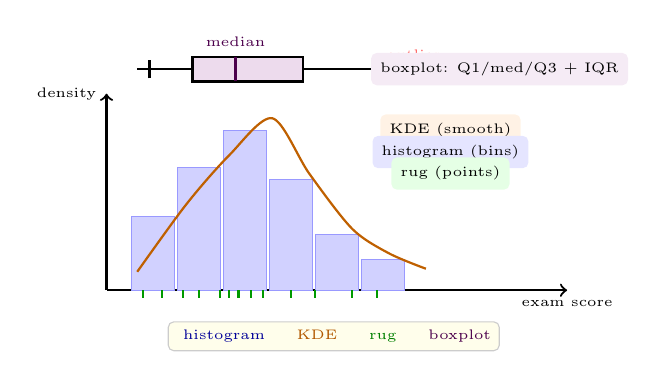
\begin{tikzpicture}[scale=0.78,every node/.style={font=\scriptsize}]
% axes
\draw[->,thick] (0,0) -- (7.5,0) node[below,font=\tiny] {exam score};
\draw[->,thick] (0,0) -- (0,3.2) node[left,font=\tiny] {density};
% histogram bars (blue)
\fill[blue!18,draw=blue!40] (0.4,0) rectangle (1.1,1.2);
\fill[blue!18,draw=blue!40] (1.15,0) rectangle (1.85,2.0);
\fill[blue!18,draw=blue!40] (1.9,0) rectangle (2.6,2.6);
\fill[blue!18,draw=blue!40] (2.65,0) rectangle (3.35,1.8);
\fill[blue!18,draw=blue!40] (3.4,0) rectangle (4.1,0.9);
\fill[blue!18,draw=blue!40] (4.15,0) rectangle (4.85,0.5);
% KDE line (orange)
\draw[thick,orange!75!black,smooth] plot coordinates {(0.5,0.3) (1.3,1.4) (2.0,2.2) (2.7,2.8) (3.3,1.9) (4.0,1.0) (4.6,0.6) (5.2,0.35)};
\node[font=\tiny,fill=orange!10,rounded corners=2pt] at (5.6,2.6) {KDE (smooth)};
\node[font=\tiny,fill=blue!10,rounded corners=2pt] at (5.6,2.25) {histogram (bins)};
% rug
\foreach \x in {0.6,0.9,1.25,1.5,1.85,2.0,2.15,2.35,2.55,3.0,3.4,4.0,4.4} \draw[green!60!black,thick] (\x,0) -- (\x,-0.12);
\node[font=\tiny,fill=green!10,rounded corners=2pt] at (5.6,1.9) {rug (points)};
% boxplot on top
\begin{scope}[yshift=3.6cm]
\draw[thick] (0.5,0) -- (4.8,0);
\draw[thick,fill=violet!14] (1.4,-0.2) rectangle (3.2,0.2);
\draw[thick,violet!60!black] (2.1,-0.2) -- (2.1,0.2) node[above,font=\tiny] {median};
\draw[thick] (1.4,0) -- (0.7,0); \draw[thick] (0.7,-0.15) -- (0.7,0.15);
\draw[thick] (3.2,0) -- (4.4,0); \draw[thick] (4.4,-0.15) -- (4.4,0.15);
\fill[red!60] (5.0,0) circle (0.07) node[above,font=\tiny] {outlier};
\node[font=\tiny,fill=violet!8,rounded corners=2pt] at (6.4,0) {boxplot: Q1/med/Q3 + IQR};
\end{scope}
\node[font=\tiny,draw=gray!40,fill=yellow!8,rounded corners=2pt,inner sep=3pt] at (3.7,-0.75) {\textcolor{blue!60!black}{$\blacksquare$ histogram} \quad \textcolor{orange!70!black}{$\blacksquare$ KDE} \quad \textcolor{green!50!black}{$\blacksquare$ rug} \quad \textcolor{violet!60!black}{$\blacksquare$ boxplot}};
\end{tikzpicture}
\caption{One distribution, four views: histogram (bars), KDE (smooth orange line), rug (ticks), and boxplot (top). Bin width and bandwidth control bias vs variance.}
\label{fig:distribution}
\end{figure}

\paragraph{Bias--variance in pictures.} Wider bins / larger $h$ lower variance but blur true modes (bias); narrower bins show sampling noise (variance). Overlay all three---bars, KDE, rug---when in doubt: the rug keeps you honest.

% ============================================================
\section{Showing Many Variables}
\label{sec:many-vars}
\paragraph{Intuition.} Two variables invite a scatterplot; three invite colour or size; ten invite a wall of views. The challenge is not drawing but \emph{comparing}: can eyes compare distributions across groups and relationships across pairs?

Two families: \emph{scatterplot matrix (SPLOM)} shows every pair as a small scatterplot---good for up to $\sim 8$ variables, then clutter dominates. \emph{Parallel coordinates} draw each variable as a vertical axis and each item as a polyline crossing them---good for spotting clusters and outliers across many dimensions, weakened by axis ordering and overplotting (rescued by bundling, opacity, and reordering).

\begin{figure}[h]\centering
\begin{tikzpicture}[scale=0.74,every node/.style={font=\scriptsize}]
% SPLOM sketch 3x3
\begin{scope}
\node[font=\footnotesize\bfseries] at (1.8,4.2) {SPLOM (pairs)};
\foreach \i in {0,1,2} \foreach \j in {0,1,2} {
  \draw[gray!40] (0.1+1.22*\i,0.1+1.22*\j) rectangle +(1.1,1.1);
  \ifnum\i=\j \node[font=\tiny] at (0.65+1.22*\i,0.65+1.22*\j) {var \i};
  \else \foreach \k in {1,...,7} {
    \pgfmathsetmacro{\rx}{rand*0.7+0.3} \pgfmathsetmacro{\ry}{rand*0.7+0.3}
    \fill[blue!55] (0.25+1.22*\i+0.6*\rx,0.25+1.22*\j+0.6*\ry) circle (0.05);
  } \fi
}
\node[font=\tiny,fill=blue!8,rounded corners=2pt] at (1.8,-0.4) {diagonal = label; off-diag = scatterplot};
\end{scope}
% parallel coordinates
\begin{scope}[xshift=5.2cm]
\node[font=\footnotesize\bfseries] at (2.2,4.2) {Parallel coordinates};
\foreach \x in {0,1.5,3.0,4.5} \draw[thick,gray!60] (\x,0) -- (\x,3.6);
\foreach \x/\lbl in {0/A,1.5/B,3.0/C,4.5/D} \node[font=\tiny] at (\x,3.85) {\lbl};
\foreach \a/\b/\c/\d/\col in {0.6/1.8/1.0/2.4/blue,0.9/2.6/2.0/1.2/red,0.4/1.2/0.6/3.0/green,1.1/2.0/1.6/2.0/orange,0.7/2.2/1.4/1.6/violet,0.5/1.5/0.8/2.8/teal} {
  \draw[thick,\col!70,opacity=0.7] (0,\a) -- (1.5,\b) -- (3.0,\c) -- (4.5,\d);
}
\node[font=\tiny,fill=orange!10,rounded corners=2pt] at (2.2,-0.4) {polyline per item; crossings show correlation};
\end{scope}
% brushing linking sketch
\begin{scope}[xshift=10.6cm]
\node[font=\footnotesize\bfseries] at (1.7,4.2) {Brushing + linking};
\draw[gray!40] (0,1.8) rectangle (1.6,3.6); \draw[gray!40] (1.9,1.8) rectangle (3.5,3.6);
\foreach \x/\y in {0.4/2.8,0.7/2.4,1.0/3.0,0.5/2.2,1.2/2.6} \fill[blue!50] (\x,\y) circle (0.06);
\foreach \x/\y in {0.6/2.6,0.8/2.9,1.1/2.5} \fill[red!70] (\x,\y) circle (0.06);
% brush rect
\draw[thick,fill=yellow!16,draw=orange!70!black] (0.45,2.45) rectangle (1.15,3.1);
\node[font=\tiny,fill=yellow!12,rounded corners=2pt] at (0.8,1.55) {brush};
% histogram below linked
\draw[gray!40] (0,0.2) rectangle (3.5,1.4);
\fill[blue!18,draw=blue!40] (0.2,0.2) rectangle (0.7,0.9);
\fill[red!30,draw=red!50] (0.75,0.2) rectangle (1.25,1.2);
\fill[blue!18,draw=blue!40] (1.3,0.2) rectangle (1.8,0.7);
\draw[thick,red!60!black,->,>=Stealth] (0.8,1.4) -- (1.0,1.8) node[midway,right,font=\tiny] {linked};
\end{scope}
\node[font=\tiny,draw=gray!40,fill=yellow!8,rounded corners=2pt,inner sep=3pt] at (6.2,-0.85) {\textcolor{blue!60!black}{$\blacksquare$ scatterplot} \quad \textcolor{red!60!black}{$\blacksquare$ brushed} \quad \textcolor{yellow!60!black}{$\blacksquare$ brush} \quad \textcolor{violet!60!black}{$\blacksquare$ polyline}};
\end{tikzpicture}
\caption{Multivariate: scatterplot matrix (left) shows all pairs; parallel coordinates (centre) show all variables as axes; brushing a scatterplot highlights linked points in a histogram (right).}
\label{fig:multivariate-interaction}
\end{figure}

% ============================================================
\section{Interaction: From Picture to Dialogue}
\label{sec:interaction}
\paragraph{Intuition.} A static chart answers one question. An interactive chart lets the reader ask the next one: ``what if I filter to 2023?'' ``who are those outliers?'' Interaction turns the pipeline into a loop where the reader steers data transforms and view parameters directly.

\begin{definition}[Shneiderman mantra and interactions]\label{def:interaction}
\emph{Overview first, zoom and filter, then details on demand.} Primitive interactions: \emph{navigate} (pan/zoom), \emph{select} (brush: rectangular, lasso), \emph{filter} (sliders, checkboxes), \emph{link} (selection in one view highlights same items elsewhere), \emph{aggregate} (change binning/level of detail), \emph{annotate} (tooltip, label on hover). \emph{Dynamic queries} update views continuously as sliders move (latency target $<100$\,ms).
\end{definition}

\begin{example}[Brushing and linking]\label{ex:brushing}
A scatterplot of price vs mileage and a histogram of price share the same items. Dragging a rectangle (brush) in the scatterplot selects points; the histogram re-colours its bins to show the selection's price distribution. Two views, one selection, instant feedback. Without linking, the reader must memorise and cross-reference.
\end{example}

\begin{remark}[Linking as coordination]\label{rem:linking}
Linking is a coordination of views, not just two charts side by side. The selection is a shared data predicate; every view that listens to it updates. This is why Altair/D3 model selections as first-class objects rather than per-chart state.
\end{remark}

Latency matters. $>500$\,ms breaks flow; $<100$\,ms feels direct. Scalability tricks: aggregate before rendering (bin, sample, or summarise), use canvas/WebGL for many marks, debounce slider events, and precompute indexed selections.

% ============================================================
\section{Visual Scalability}
\label{sec:scalability}
Even with fast interaction, eyes have limits. Overplotting hides structure once marks exceed $\sim$10k visible points; aggregation (hexbin, 2-D histogram, contour) trades detail for legibility. For high-cardinality nominal splits, small multiples beat colour overload (eyes hold $\sim$7 colours in working memory). When rows reach millions, server-side binning with client-side brushing keeps latency flat; the picture shows summaries, the interaction reveals individuals on demand.

\begin{lstlisting}[language=Python, caption={Histogram vs KDE and bandwidth choice with NumPy/Matplotlib.}, label={lst:hist-kde}]
import numpy as np, matplotlib.pyplot as plt

np.random.seed(0)
x = np.concatenate([np.random.normal(0,1,220), np.random.normal(4,0.8,80)])
for bins in [8, 30]:
    plt.figure(); plt.hist(x, bins=bins, density=True, color="steelblue", alpha=0.5, edgecolor="white")
    plt.title(f"Histogram bins={bins}"); plt.savefig(f"hist{bins}.pdf")
# KDE with two bandwidths
from scipy.stats import gaussian_kde
for bw in [0.2, 1.0]:
    kde = gaussian_kde(x, bw_method=bw)
    xs = np.linspace(-3, 7, 400)
    plt.figure(); plt.plot(xs, kde(xs), color="orangered", lw=2)
    plt.title(f"KDE bw={bw}"); plt.savefig(f"kde{bw}.pdf")
\end{lstlisting}

\begin{lstlisting}[language=Python, caption={Brushing and linking with Altair selections.}, label={lst:altair-brush}]
import altair as alt, pandas as pd, numpy as np
np.random.seed(1)
df = pd.DataFrame({"price": np.random.lognormal(3,0.5,300),
                   "mileage": np.random.normal(50,15,300)})
brush = alt.selection_interval(name="brush")
scatter = alt.Chart(df).mark_point().encode(
    x="mileage:Q", y="price:Q", color=alt.condition(brush, alt.value("orangered"), alt.value("steelblue"))
).add_params(brush).properties(width=260, height=180)
hist = alt.Chart(df).mark_bar().encode(
    x=alt.X("price:Q", bin=alt.Bin(maxbins=20)), y="count()",
    color=alt.condition(brush, alt.value("orangered"), alt.value("lightgray"))
).transform_filter(brush).properties(width=260, height=100)
chart = alt.vconcat(scatter, hist)
chart  # in a notebook, drag on the scatterplot to see the linked histogram update
\end{lstlisting}

% ============================================================
\section{Chapter Notes}
% Notes on statistical charts and interaction
Cleveland (1993) and Wilkinson (Grammar of Graphics, 2005) grounded statistical charts; Scott and Freedman--Diaconis gave principled bin widths; Shneiderman (1996) articulated the mantra and dynamic queries; Becker and Cleveland's brushing (1987) and Buja et al.\ linking remain the interaction canon; Heer and Shneiderman (2012) surveyed interactive dynamics. The next chapter scales these ideas to networks.

% ============================================================
\section{Exercises}
\label{sec:ch04-exercises}
\begin{enumerate}[label=E4.\arabic*, leftmargin=*, itemsep=0.8em]
    \item \textbf{Bin rules.} For $n=500$, $\sigma=12$, IQR$=10$, compute Sturges $k$, Scott $h$, and Freedman--Diaconis $h$. Convert $h$ to $k$ for range 0--100. Which rule is most robust to outliers and why?
    \item \textbf{Bandwidth trade-off.} Given a bimodal mixture $0.7N(0,1)+0.3N(4,0.8)$, sketch KDEs at $h=0.2,0.6,1.5$. Label where the second mode disappears (bias) and where wiggles appear (variance).
    \item \textbf{SPLOM vs parallel coordinates.} For a 6-variable dataset, list one question answered faster by a SPLOM and one faster by parallel coordinates. Propose axis ordering and opacity settings to reduce clutter in the parallel-coordinates view.
    \item \textbf{Build brushing.} Using Altair (or D3), implement the price vs mileage brushing in Listing~\ref{lst:altair-brush} and add a second slider that filters by year. Report interaction latency strategy if the table grew to $10^6$ rows.
    \item \textbf{Details on demand.} Design a tooltip and a side-panel details view for a scatterplot outlier. What attributes go in the tooltip (immediate) vs the panel (on click), and why? Justify with the mantra and with latency/accessibility.
\end{enumerate}
% End of Chapter 4
% pad
